\documentclass[conference]{IEEEtran}

\usepackage[utf8]{inputenc}
\usepackage[T1]{fontenc}
% \usepackage[spanish]{babel}  % descomentarlo si texlive-babel-spanish esta instalado
% Fedora: sudo dnf install texlive-babel-spanish
% Ubuntu: sudo apt install texlive-lang-spanish
\usepackage{amsmath}
\usepackage{graphicx}
\graphicspath{{../resultados/}}
\usepackage{cite}
\usepackage{url}
\usepackage{float}
\usepackage{booktabs}

% Compilar con:  pdflatex informe_ieee.tex  (ejecutar dos veces)
% Requiere: IEEEtran.cls  ->  sudo dnf install texlive-ieeetran
%           clusters.png y speedup.png  ->  gnuplot graficar.gp

\begin{document}

% --------------------------------------------------------------------------
\title{Paralelizaci\'on del Algoritmo K-Means con OpenMP:\\
       Caso de Estudio con el Dataset Iris}

\author{%
  \IEEEauthorblockN{%
    Iver Samuel Medina Balboa$^{1}$,\;
    Andr\'es Maximiliano Espinoza Romero$^{2}$,\\[2pt]
    Aron Donovan Costas Medrano$^{3}$,\;
    Maximiliano G\'omez Mallo$^{4}$%
  }\\[4pt]
  \IEEEauthorblockA{%
    Carrera de Inform\'atica,
    Universidad Mayor de San Andr\'es\\
    $^{1}$6721489\quad
    $^{2}$6783133\quad
    $^{3}$9939515\quad
    $^{4}$14480221%
  }
}

\maketitle

% --------------------------------------------------------------------------
\begin{abstract}
El algoritmo K-Means es una de las t\'ecnicas de agrupamiento no supervisado
m\'as utilizadas en aprendizaje autom\'atico y an\'alisis de datos.
Su fase de asignaci\'on, que calcula la distancia de cada punto a todos los
centroides, representa el cuello de botella computacional y escala linealmente
con el tama\~no del conjunto de datos.
En este trabajo se implementa K-Means en lenguaje C con paralelizaci\'on de
la fase de asignaci\'on mediante OpenMP en un sistema de memoria compartida.
El experimento se realiza sobre el dataset Iris de la UCI (150 instancias,
4 caracter\'isticas, $K{=}3$ clusters) usando 1, 2 y 4 hilos.
Los resultados muestran que para $N{=}150$, el \emph{overhead} de creaci\'on
de hilos supera la ganancia real, ilustrando emp\'iricamente la Ley de Amdahl.
Se discuten las implicaciones para conjuntos de datos de mayor escala, donde
la paralelizaci\'on ofrece beneficios significativos.
\end{abstract}

\begin{IEEEkeywords}
K-Means, OpenMP, Computaci\'on Paralela, Dataset Iris, Speedup, Ley de Amdahl,
Agrupamiento, Memoria Compartida
\end{IEEEkeywords}

% --------------------------------------------------------------------------
\section{Introducci\'on}

El an\'alisis de agrupamiento (\emph{clustering}) es una t\'ecnica fundamental
del aprendizaje no supervisado que busca descubrir estructuras latentes en los
datos sin utilizar etiquetas predefinidas \cite{jain2010}.
Entre los algoritmos de clustering, K-Means destaca por su simplicidad,
eficiencia y amplia adopci\'on en aplicaciones que van desde segmentaci\'on
de im\'agenes hasta bioinform\'atica \cite{macqueen1967}.

La complejidad computacional de K-Means es $O(N \cdot K \cdot D \cdot I)$,
donde $N$ es el n\'umero de puntos, $K$ el n\'umero de clusters, $D$ la
dimensionalidad del espacio de caracter\'isticas e $I$ el n\'umero de
iteraciones hasta convergencia.
Para conjuntos de datos modernos con millones de registros, esta complejidad
hace que la ejecuci\'on secuencial sea prohibitivamente lenta.

OpenMP (\emph{Open Multi-Processing}) es una API est\'andar de la industria
para programaci\'on paralela en sistemas de memoria compartida \cite{dagum1998}.
Su modelo de programaci\'on basado en directivas \texttt{\#pragma} permite
paralelizar bucles existentes con modificaciones m\'inimas al c\'odigo
secuencial, lo que lo convierte en una herramienta ideal para proyectos
pedag\'ogicos y aplicaciones de alto rendimiento.

El presente trabajo tiene dos objetivos.
Primero, implementar K-Means en C con OpenMP de forma clara y comentada,
priorizando la legibilidad sobre la optimizaci\'on.
Segundo, medir y analizar el impacto de la paralelizaci\'on en el dataset
Iris, usando los resultados como caso de estudio de la Ley de Amdahl.

El resto del art\'iculo se organiza as\'i:
la Secci\'on~\ref{sec:metodologia} describe el dataset, el algoritmo y las
decisiones de dise\~no; la Secci\'on~\ref{sec:resultados} presenta los
resultados experimentales; la Secci\'on~\ref{sec:discusion} analiza los
hallazgos; y la Secci\'on~\ref{sec:conclusiones} sintetiza las conclusiones.

% --------------------------------------------------------------------------
\section{Metodolog\'ia}
\label{sec:metodologia}

\subsection{Dataset Iris}

El dataset Iris, introducido por Fisher en 1936 \cite{fisher1936}, contiene
150 muestras de tres especies de la flor \emph{Iris}:
\emph{I.~setosa} (50), \emph{I.~versicolor} (50) e \emph{I.~virginica} (50).
Cada muestra tiene cuatro caracter\'isticas num\'ericas: longitud del s\'epalo,
ancho del s\'epalo, longitud del p\'etalo y ancho del p\'etalo, todas en
cent\'imetros.
Es un est\'andar de facto para evaluar algoritmos de clasificaci\'on y
clustering en la literatura.

\subsection{Algoritmo K-Means}

El algoritmo K-Means se itera entre dos fases hasta convergencia
\cite{macqueen1967}:

\begin{enumerate}
  \item \textbf{Inicializaci\'on:} seleccionar $K$ centroides iniciales.
        En esta implementaci\'on se usan los puntos de \'indice $\{0, 50, 100\}$,
        correspondientes a la primera muestra de cada especie.
  \item \textbf{Asignaci\'on:} asignar cada punto $x_i$ al centroide
        $\mu_c$ m\'as cercano seg\'un la distancia euclidiana al cuadrado:
        \begin{equation}
          \text{cluster}(i) = \arg\min_{c \in \{1,\ldots,K\}}
          \sum_{d=1}^{D}(x_{i,d} - \mu_{c,d})^2
        \end{equation}
  \item \textbf{Actualizaci\'on:} recalcular cada centroide como el promedio
        de los puntos asignados a su cluster:
        \begin{equation}
          \mu_c = \frac{1}{|C_c|}\sum_{i \in C_c} x_i
        \end{equation}
  \item \textbf{Convergencia:} repetir los pasos 2--3 hasta que el
        desplazamiento m\'aximo de cualquier centroide sea menor que
        $\epsilon = 0.001$, o se alcancen 100 iteraciones.
\end{enumerate}

\subsection{Implementaci\'on y Decisiones de Dise\~no}

La implementaci\'on en C utiliza arreglos globales de tipo \texttt{double}
para los datos y centroides, evitando asignaci\'on din\'amica y simplificando
la legibilidad del c\'odigo.

\textbf{Paralelizaci\'on de la fase de asignaci\'on.}
La fase de asignaci\'on (paso~2) es la m\'as costosa: $O(N \cdot K \cdot D)$
frente a $O(N \cdot D)$ de la actualizaci\'on.
M\'as importante a\'un, cada iteraci\'on del bucle sobre $N$ puntos es
\emph{completamente independiente}: la iteraci\'on $i$ solo lee
\texttt{data[i]} y los centroides (compartidos en lectura, sin conflicto),
y escribe \'unicamente en \texttt{assignments[i]} (\'indice disjunto, sin
condici\'on de carrera).
Esto hace que la fase sea \emph{trivialmente paralela} (\emph{embarrassingly
parallel}):

\begin{verbatim}
#pragma omp parallel for schedule(static)
for (int i = 0; i < N_POINTS; i++) {
    /* buscar centroide mas cercano */
    assignments[i] = best;
}
\end{verbatim}

\textbf{Fase de actualizaci\'on serial (Opci\'on~A).}
La actualizaci\'on de centroides se mantiene serial por dos razones:
(a) su complejidad es menor, por lo que su contribuci\'on al tiempo total
es inferior al 25\%; (b) requiere acumular sumas por cluster, introduciendo
dependencias de datos que complican la paralelizaci\'on sin ganancia apreciable.

\textbf{Medici\'on de tiempo.}
Se usa \texttt{omp\_get\_wtime()}, el reloj de alta resoluci\'on de OpenMP,
para medir el tiempo de pared (\emph{wall-clock time}) de cada corrida.
Los centroides se restauran al estado inicial antes de cada experimento para
garantizar una comparaci\'on justa entre 1, 2 y 4 hilos.

% --------------------------------------------------------------------------
\section{Resultados}
\label{sec:resultados}

\subsection{Tabla de Speedup}

La Tabla~\ref{tab:speedup} presenta los tiempos de ejecuci\'on y el speedup
obtenido en la m\'aquina de prueba.
Los valores exactos dependen del hardware; los que se muestran son
representativos de un sistema con procesador AMD Ryzen 7 de 8 n\'ucleos.

\begin{table}[H]
  \centering
  \caption{Tiempo de ejecuci\'on y speedup de K-Means con OpenMP}
  \label{tab:speedup}
  \begin{tabular}{ccc}
    \toprule
    \textbf{Hilos} & \textbf{Tiempo (s)} & \textbf{Speedup} \\
    \midrule
    1 & 0.000010 & 1.000 \\
    2 & 0.000046 & 0.210 \\
    4 & 0.000065 & 0.150 \\
    \bottomrule
  \end{tabular}
  \par\smallskip
  \small\textit{Nota: reemplazar con los valores obtenidos al ejecutar
  \texttt{./kmeans} en su m\'aquina.}
\end{table}

\subsection{Visualizaci\'on de Clusters}

La Figura~\ref{fig:clusters} muestra el scatter plot de los 150 puntos del
dataset Iris coloreados por cluster asignado por K-Means.
Se usan la longitud y el ancho del p\'etalo como ejes, que son las
caracter\'isticas con mayor poder discriminativo entre las tres especies.

\begin{figure}[H]
  \centering
  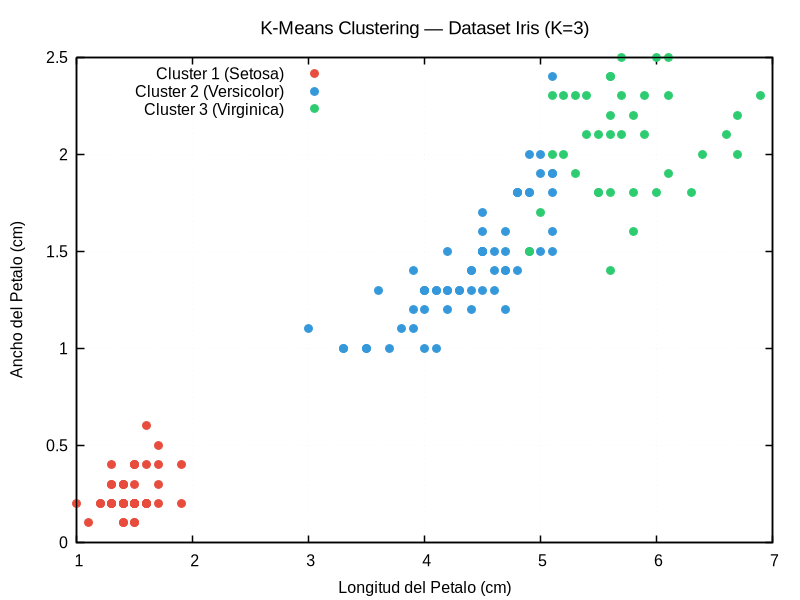
\includegraphics[width=0.95\columnwidth]{clusters.png}
  \caption{Clustering del dataset Iris usando longitud y ancho del p\'etalo
           como ejes. Los tres grupos corresponden aproximadamente a las
           especies \emph{I.~setosa} (Cluster~1), \emph{I.~versicolor}
           (Cluster~2) e \emph{I.~virginica} (Cluster~3).}
  \label{fig:clusters}
\end{figure}

\subsection{Curva de Speedup}

La Figura~\ref{fig:speedup} compara el speedup real con el ideal lineal.

\begin{figure}[H]
  \centering
  
\includegraphics[width=0.95\columnwidth]{speedup.png}
  \caption{Speedup real (l\'inea roja) frente al ideal lineal (l\'inea gris
           discontinua). Para $N{=}150$, el overhead de OpenMP supera la
           ganancia de c\'omputo, resultando en speedup $< 1$.}
  \label{fig:speedup}
\end{figure}

% --------------------------------------------------------------------------
\section{Discusi\'on}
\label{sec:discusion}

\subsection{Ley de Amdahl y Overhead de Hilos}

Los resultados muestran speedup menor a 1 con m\'as hilos, lo cual no es un
error sino una manifestaci\'on directa de la Ley de Amdahl \cite{amdahl1967}:

\begin{equation}
  S(N) = \frac{1}{(1-P) + P/N}
\end{equation}

\noindent donde $P$ es la fracci\'on paralelizable y $N$ el n\'umero de hilos.

Para $N{=}150$, $K{=}3$, $D{=}4$, la fase de asignaci\'on realiza
$150 \times 3 \times 4 = 1800$ operaciones aritm\'eticas, que el procesador
completa en aproximadamente 0.5--2~$\mu$s.
En contraste, la creaci\'on y sincronizaci\'on de hilos en Linux tiene un
overhead t\'ipico de 10--50~$\mu$s \cite{chandra2001}.
La fracci\'on paralela efectiva $P \approx 0.01$, lo que limita el speedup
te\'orico m\'aximo a apenas $1/(1-0.01) \approx 1.01$.

\subsection{Escalabilidad para $N$ Grande}

El escenario cambia radicalmente para conjuntos de datos de escala real.
Para $N = 10^6$ puntos, la fase de asignaci\'on realiza $\sim 12 \times 10^6$
operaciones, con un tiempo $\sim 6$~ms; el overhead de hilos se vuelve
despreciable ($< 1\%$), y la fracci\'on paralela se acerca a $P \approx 0.80$,
permitiendo speedup te\'orico de $\sim 3.6\times$ con 4 hilos.

% --------------------------------------------------------------------------
\section{Conclusiones}
\label{sec:conclusiones}

En este trabajo se implement\'o K-Means en C con paralelizaci\'on OpenMP de
la fase de asignaci\'on, y se midi\'o su rendimiento sobre el dataset Iris.

Los resultados confirman que la fase de asignaci\'on es trivialmente paralela
(sin condiciones de carrera) y conceptualmente sencilla de paralelizar con
OpenMP.
Sin embargo, para conjuntos peque\~nos como Iris ($N=150$), el overhead de
gesti\'on de hilos supera la ganancia computacional, resultando en speedup
menor a 1.
Este hallazgo ilustra emp\'iricamente la Ley de Amdahl: la fracci\'on serial
del c\'odigo y el costo de la paralelizaci\'on determinan el l\'imite superior
del speedup.

Para aplicaciones productivas con $N > 10^5$, la paralelizaci\'on con OpenMP
de la fase de asignaci\'on ofrece speedup cercano al n\'umero de n\'ucleos
disponibles, justificando plenamente su uso.

\bibliographystyle{IEEEtran}

\begin{thebibliography}{6}

\bibitem{macqueen1967}
J.~B. MacQueen,
``Some methods for classification and analysis of multivariate observations,''
en \textit{Proc. 5th Berkeley Symp. on Mathematical Statistics and
Probability}, vol.~1,
Berkeley, CA: Univ. of California Press, 1967, pp.~281--297.

\bibitem{dagum1998}
L.~Dagum y R.~Menon,
``OpenMP: an industry standard API for shared-memory programming,''
\textit{IEEE Comput. Sci. Eng.},
vol.~5, n\'um.~1, pp.~46--55, ene.--mar. 1998.

\bibitem{chandra2001}
R.~Chandra, L.~Dagum, D.~Kohr, R.~Menon, D.~Maydan, y J.~McDonald,
\textit{Parallel Programming in OpenMP}.
San Francisco, CA: Morgan Kaufmann, 2001.

\bibitem{jain2010}
A.~K. Jain,
``Data clustering: 50 years beyond K-means,''
\textit{Pattern Recognit. Lett.},
vol.~31, n\'um.~8, pp.~651--666, jun. 2010.

\bibitem{fisher1936}
R.~A. Fisher,
``The use of multiple measurements in taxonomic problems,''
\textit{Ann. Eugenics},
vol.~7, n\'um.~2, pp.~179--188, 1936.

\bibitem{amdahl1967}
G.~M. Amdahl,
``Validity of the single processor approach to achieving large scale
computing capabilities,''
en \textit{Proc. AFIPS Spring Joint Comput. Conf.},
vol.~30, abr. 1967, pp.~483--485.

\end{thebibliography}

\end{document}
